\documentclass[11pt]{article}

% ---------- packages ----------
\usepackage[a4paper,margin=1in]{geometry}
\usepackage{amsmath,amssymb,mathtools}
\usepackage{bm}
\usepackage{booktabs}
\usepackage{graphicx}
\usepackage{array}
\usepackage{enumitem}
\usepackage{xcolor}
\usepackage{listings}
\usepackage{caption}
\usepackage{hyperref}

% ---------- colours ----------
\definecolor{NavyBlue}{RGB}{26,72,140}
\definecolor{CodeBg}{RGB}{246,248,251}
\definecolor{CodeKw}{RGB}{45,95,208}
\definecolor{CodeCm}{RGB}{120,132,148}
\definecolor{TodoBg}{RGB}{255,244,222}
\definecolor{TodoBd}{RGB}{178,106,28}
\hypersetup{colorlinks=true,linkcolor=NavyBlue,citecolor=NavyBlue,urlcolor=NavyBlue}

% ---------- listings style ----------
\lstdefinestyle{ep}{
  backgroundcolor=\color{CodeBg},
  basicstyle=\ttfamily\small,
  keywordstyle=\color{CodeKw}\bfseries,
  commentstyle=\color{CodeCm}\itshape,
  numberstyle=\tiny\color{CodeCm},
  frame=single, framerule=0pt, rulecolor=\color{CodeBg},
  showstringspaces=false, breaklines=true,
  columns=fullflexible, keepspaces=true,
  xleftmargin=1em, xrightmargin=1em, aboveskip=1em, belowskip=1em,
}
\lstset{style=ep,language=C++}

% ---------- a visible TODO box for the not-yet-done sections ----------
\newcommand{\todo}[1]{%
  \par\vspace{4pt}\noindent
  \fcolorbox{TodoBd}{TodoBg}{\parbox{\dimexpr\linewidth-2\fboxsep-2\fboxrule}{%
  \textbf{\color{TodoBd}TO BE ADDED.}~#1}}\vspace{4pt}\par}

% ---------- math shorthands ----------
\newcommand{\E}{\mathbb{E}}
\newcommand{\QQ}{\mathbb{Q}}
\newcommand{\dd}{\mathrm{d}}
\newcommand{\DF}{\mathrm{DF}}
\newcommand{\ind}[1]{\mathbf{1}\{#1\}}
\newcommand{\Lh}{\mathcal{L}_h}
\DeclareMathOperator*{\argmin}{arg\,min}

\captionsetup{font=small,labelfont=bf}
\setlength{\emergencystretch}{2em}   % absorb the last few pt of long unbreakable names (no overfull)

% ---------- title ----------
\title{\vspace{-1.5em}\textbf{Pricing an Equity Accumulator with Daily Knock-Out}\\[0.3em]
\large A Local-Volatility Finite-Difference Engine\\[0.2em]
\normalsize Underlying: Galaxy Entertainment (0027.HK)}
\author{Zhizu Li}
\date{\today}

\begin{document}
\maketitle
\vspace{-1em}

\begin{abstract}
\noindent
We price a one-year, physically settled share accumulator on Galaxy Entertainment (0027.HK). The contract includes a daily up-and-out knock-out feature. The contract is Markovian in the single underlying. The daily accrual is an additive strip of forwards rather than a path-dependent state variable. The knock-out is an absorbing barrier. These features make a one-dimensional finite-difference scheme both accurate and efficient. Our primary pricing engine uses a
\textbf{Crank--Nicolson PDE} solver in log-spot space. The engine supports both Black--Scholes and
local volatility. It handles the daily discrete barrier exactly. It also incorporates the contract’s guaranteed-delivery period and accrual cap. We validate the engine against an independent closed-form \textbf{Reiner--Rubinstein} benchmark. Under matched constant volatility, the PDE converges to this benchmark in the continuous-monitoring limit. We also use the
\textbf{Broadie--Glasserman--Kou} shift to illustrate the correction for discrete barrier monitoring. We also build a toy Monte Carlo model to verify our PDE approach. The market data are built from the
\textbf{HKD OIS curve} and
\textbf{option-implied forwards}. The volatility layer uses an arbitrage-free \textbf{SSVI}
surface and the corresponding \textbf{Dupire} local volatility. We use the actual trade-date market
data (2024-11-06; Bloomberg \texttt{ICVS}~145, \texttt{OVME}, \texttt{OVDV}). On that market the
accumulator is worth about $-39.9$k HKD under Black--Scholes and about $-46.0$k under local
volatility.
\end{abstract}

\tableofcontents
\bigskip

% =====================================================================
\section{The Instrument}\label{sec:instrument}
% =====================================================================

\subsection{Contract terms}
Table~\ref{tab:terms} summarises the economically relevant terms.

\begin{table}[h]
\centering
\small
\begin{tabular}{@{}lll@{}}
\toprule
\textbf{Field} & \textbf{Value} & \textbf{Role} \\
\midrule
Underlying               & Galaxy Entertainment 0027.HK (HKD) & spot process $S_t$ \\
Forward (accrual) price  & $K = 31.0804$ & fixed purchase price \\
Knock-out price          & $H = 37.1825$ & up-and-out barrier \\
Barrier monitoring       & each scheduled trading day (close) & \emph{discrete, daily} \\
Daily number of shares   & $N = 234$ & accrual quantity \\
Max scheduled days       & $245$ & accrual cap \\
Trade / Start date       & 2024-11-06 / 2024-11-07 & \\
Final valuation date     & 2025-11-05 & horizon $\approx 1$\,yr \\
Guaranteed delivery      & through 2024-12-04 & minimum-accrual floor \\
Settlement               & physical, $\sim$26 fortnightly periods & delivery of shares \\
Initial exchange         & Citi $\to$ Counterparty HKD $23{,}906.61$ & upfront payment \\
\bottomrule
\end{tabular}
\caption{Term-sheet parameters of Deal H19871600A.}
\label{tab:terms}
\end{table}

\subsection{Taxonomy and classification}
Following Lam, Yu \& Xin (2009), we characterise an accumulator along three independent dimensions:
\begin{enumerate}[leftmargin=1.5em,itemsep=1pt]
  \item \textbf{Gearing $g$}: This parameter determines the multiplier on the put leg. A typical accumulator has
        $g=2$, which results in double accrual below the strike. our contract has \textbf{$g=1$}, which means that the daily quantity remains constant.
  \item \textbf{Barrier monitoring}: The barrier can be monitored either continuously or discretely. Our contract is monitored at daily closes, so it has a discrete barrier.
  \item \textbf{Settlement}: The contract can settle either immediately or with a delay. Our contract settles physically on a fortnightly delayed schedule.
\end{enumerate}
Our deal is therefore an \emph{ungeared, discrete-barrier, delay-settled, physical accumulator}.
The deal also contains two features beyond the standard taxonomy: a guaranteed-delivery period and an accrual cap. We extend the model to incorporate local volatility.

\subsection{Economic decomposition}
On each live observation day, the buyer receives a forward payoff. For $g=1$,
this payoff equals $S_{t_i}-K$. We can split it into two pieces. It is a long
up-and-out call minus a long up-and-out put. Both legs are struck at $K$ and
share the barrier $H$.

% =====================================================================
\section{Market Data}\label{sec:data}
% =====================================================================
All inputs come from a real Bloomberg. We take the data on the \textbf{trade date,
2024-11-06}. The spot is $S_0=34.50$~HKD. This is the OVDV surface reference. The discount and forward curves drive the engine. We build the arbitrage-free
volatility surface and its local volatility later, in Section~\ref{sec:market}.

\subsection{HKD OIS discount curve}
Discounting uses the HKD \textbf{OIS} curve (Bloomberg \texttt{ICVS} curve~145, Settle
11/06/24, Mid), Table~\ref{tab:ois}.

\begin{table}[h]\centering\small
\begin{tabular}{@{}lrr@{}}
\toprule
Date & $z(T)$ (\%) & $\DF(T)$ \\
\midrule
2025-05-08 & 3.2915 & 0.98363 \\
2025-08-08 & 3.4752 & 0.97416 \\
2025-11-10 & 3.0658 & 0.96948 \\
2026-11-09 & 3.0269 & 0.94102 \\
2027-11-08 & 2.9142 & 0.91614 \\
\bottomrule
\end{tabular}
\caption{HKD OIS pillars: continuously-compounded ACT/365 zero rates and quoted discount factors.}
\label{tab:ois}
\end{table}

We reproduce Bloomberg's \emph{Step Forward (Cont)} stripping. In that scheme the instantaneous
forward rate is piecewise constant. Equivalently, the \emph{time-weighted zero}
$w(T)\equiv z(T)\,T=-\ln\DF(T)$ is interpolated \textbf{linearly} in $T$, with $w(0)=0$. The
discount factor is then log-linear:
\begin{equation}
  \DF(T)=e^{-w(T)},\qquad
  w(T)=w(T_i)+\frac{T-T_i}{T_{i+1}-T_i}\bigl(w(T_{i+1})-w(T_i)\bigr),\quad T\in[T_i,T_{i+1}].
  \label{eq:dfinterp}
\end{equation}


\subsection{Forward from a two-curve carry}
We do not interpolate the forward directly. Instead we \emph{reconstruct} it from two curves: a
funding-rate curve and an implied-dividend curve. Both come from Bloomberg \texttt{OVME} on
\texttt{27 HK Equity}, as the per-leg \emph{HKD Rate (MMkt)} and \emph{Impl Dividends} of
Table~\ref{tab:fwd}. The forward is then
\begin{equation}
  F(T) \;=\; S_0\,\exp\!\bigl(w_r(T)-w_q(T)\bigr),\qquad
  w_r(T)=r_{\mathrm{fwd}}(T)\,T,\quad w_q(T)=q(T)\,T,
  \label{eq:fwd-carry}
\end{equation}
Here $w_r$ is the time-weighted funding zero and $w_q$ is the time-weighted dividend. We
interpolate each one piecewise-linearly in $T$, with a $(0,0)$ node, so $F(0)=S_0$. The two curves
play different roles on purpose. The funding leg $r_{\mathrm{fwd}}$ is \texttt{OVME}'s
\emph{money-market} (HIBOR) rate. That rate is what reproduces the market put--call-parity forward.
Discounting of the payoff uses the separate OIS curve of Section~\ref{sec:data}. The two rates
differ by the HIBOR--OIS basis, about $60$--$90$\,bp. Growing the forward off OIS instead would
lower it by that basis.

\begin{table}[h]\centering\small
\begin{tabular}{@{}lrrr@{}}
\toprule
Date & $r_{\mathrm{fwd}}(T)$ (\%) & $q(T)$ (\%) & $F(T)$ \\
\midrule
2025-05-08 & 4.068 & 1.909 & 34.876 \\
2025-08-08 & 3.974 & 1.270 & 35.210 \\
2025-11-10 & 3.922 & 1.969 & 35.188 \\
2026-11-09 & 3.796 & 2.143 & 35.664 \\
\bottomrule
\end{tabular}
\caption{\texttt{OVME} funding rate (MMkt) and implied dividend per leg, and the forward
reconstructed via \eqref{eq:fwd-carry} at $S_0=34.50$. }
\label{tab:fwd}
\end{table}

\subsection{Implied volatility surface}
The two models read this surface differently. The Black--Scholes engine reads one vol, at the strike
and tenor. Local volatility reads the whole surface. The input is the Bloomberg \texttt{OVDV} grid,
spot-moneyness $80\%$--$120\%$ across 16 expiries at spot $34.50$ (Figure~\ref{fig:volsurf}). 

From the surface, we identify there's a positive skew, that implies a positive SSVI correlation $\rho>0$. The second feature is how the curvature changes with maturity. The smile
is sharp at the front, but it flattens fast, and beyond about two years it is nearly flat. In SSVI
the curvature is $\phi(\theta)=\eta\,\theta^{-\gamma}$, and $\gamma$ sets how fast it decays with
maturity. A smile that flattens as fast as the no-arbitrage ceiling allows drives $\gamma$ to its
bound of $0.5$. Because $\gamma\approx0.5$, only the front of the
surface carries real structure, and the flat long end is irrelevant to a one-year trade. This is why
we calibrate on the front window (Section~\ref{sec:market}).

\begin{figure}[h]\centering
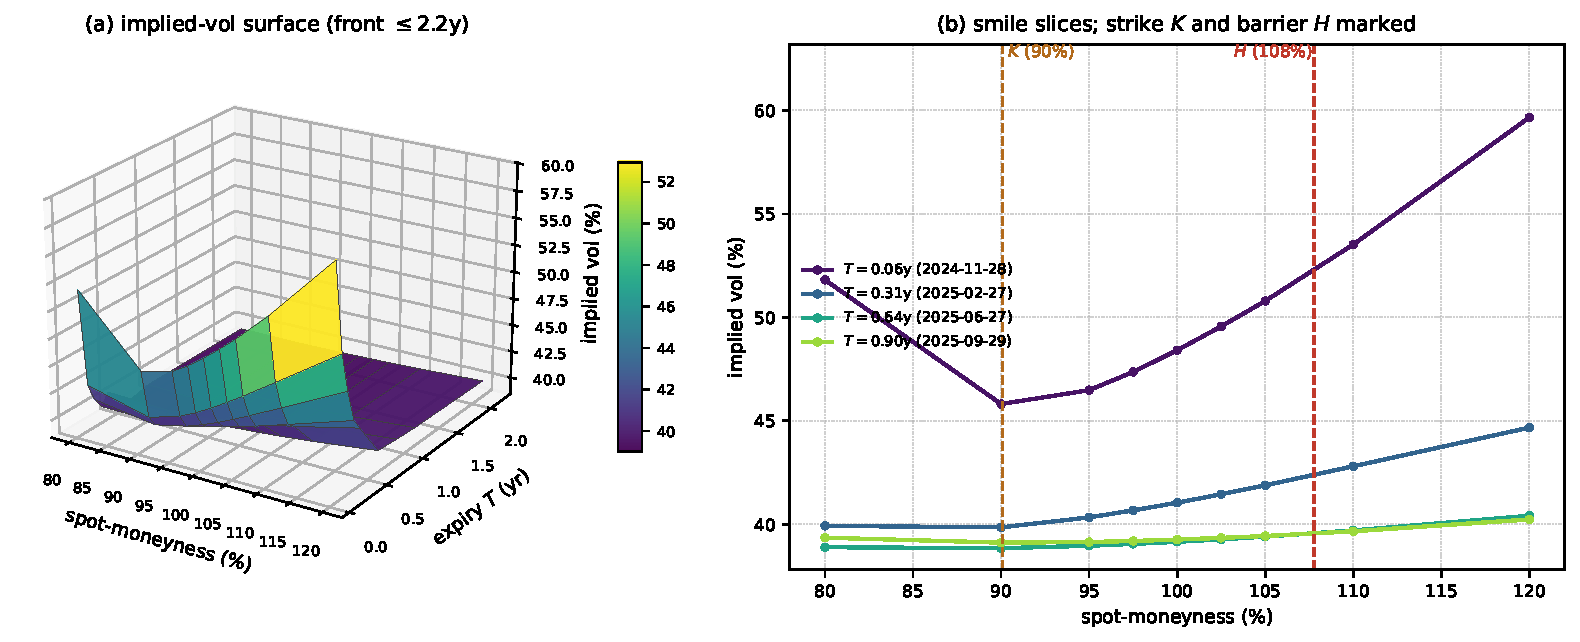
\includegraphics[width=\linewidth]{fig/vol_surface_1106.pdf}
\caption{0027.HK implied-volatility surface on the trade date (2024-11-06, \texttt{OVDV}).}
\label{fig:volsurf}
\end{figure}

% =====================================================================
\section{Pricing Framework: The Crank--Nicolson PDE Engine}\label{sec:framework}
% =====================================================================
\subsection{Choice of method}
Three schemes could price this contract: Monte Carlo, a trinomial tree, and a finite-difference
PDE. One fact decides the choice. The contract is \textbf{Markovian in the single underlying}.
The accrued quantity is not a state variable, since each day contributes only $S_{t_i}-K$. The
accrual cap is a deterministic calendar date. The guaranteed period admits a closed-form add-on.
The knock-out is an \emph{absorbing} barrier. So there is no auxiliary path-dependent dimension.
A one-dimensional PDE therefore prices the contract essentially exactly.

\paragraph{Clean, deterministic Greeks where the risk lives.} An accumulator's risk is dominated
by Gamma and Vega around the barrier. A PDE solves for the whole value surface $W(x,t)$. So
$\Delta=\partial_x W$ and $\Gamma=\partial_{xx}W$ read straight off adjacent nodes.

\paragraph{The discrete barrier is exact.} Daily monitoring coincides with the daily time steps.
The barrier $\ln H$ is aligned to a grid node. The knock-out reset is therefore exact. Each step
costs $O(N_x)$ with the Thomas algorithm, which gives a deterministic, sub-second valuation.

\subsection{Why the PDE fits local volatility}
The preferred model is local volatility. Finite differences are most natural precisely here.
\begin{itemize}[leftmargin=1.4em,itemsep=2pt]
  \item \textbf{$\sigma_{\mathrm{loc}}$ is a deterministic coefficient field on the PDE's own
  grid.} Dupire local volatility $\sigma_{\mathrm{loc}}(S,t)$ is defined at every $(S,t)$. The
  scheme evaluates it at each node $(S_j,t_k)$ as the diffusion coefficient
  $\alpha_j=\tfrac12\sigma_{\mathrm{loc}}(S_j,t_k)^2$. It drops in with no extra machinery.
  Black--Scholes is then the same engine with $\sigma$ constant, through one vol-provider interface.
  \item \textbf{Dupire is PDE-native.} Dupire's formula comes from the \emph{forward}
  (Fokker--Planck) PDE for call prices. We calibrate $\sigma_{\mathrm{loc}}$ so that the forward
  PDE reprices vanillas. We then feed the same $\sigma_{\mathrm{loc}}$ into the \emph{backward}
  PDE for the exotic. The whole pipeline stays in one consistent finite-difference framework.
\end{itemize}

\subsection{Payoff and risk-neutral value}
Take the valuation date (as-of) as $t=0$, in years. Let $t_1<\dots<t_n$ be the observation days.
Let $\DF(t)=\exp(-\int_0^t r)$ be the discount factor. A share accrued on day $t_i$ is not paid on
$t_i$. It is delivered and paid on the \emph{Settlement Date} $s(t_i)$ of its fortnightly
accumulation period. That date is the period's Valuation Date plus two HKEX clearance business days
($T{+}2$). The $(S_{t_i}-K)$ payoff is fixed at observation but discounted to settlement. Let the first knock-out time be
\begin{equation}
  \tau \;=\; \min\bigl\{\, t_j : S_{t_j}\ge H \,\bigr\}
  \qquad(\text{daily, discrete monitoring}).
\end{equation}
The as-of present value delivered to the buyer is the random variable
\begin{equation}
  X \;=\; \sum_{i=1}^{n}\DF(t_i)\,N\,(S_{t_i}-K)\,\ind{\tau> t_i},
  \label{eq:payoff}
\end{equation}
and the price is its risk-neutral expectation
\begin{equation}
  V_0 \;=\; \E^{\QQ}[X]
      \;=\; \sum_{i=1}^{n}\DF(t_i)\,N\,\E^{\QQ}\!\bigl[(S_{t_i}-K)\,\ind{\tau> t_i}\bigr].
  \label{eq:price}
\end{equation}
Under deterministic rates/dividends and local volatility, the spot follows
\begin{equation}
  \dd S_t \;=\; (r-q)\,S_t\,\dd t \;+\; \sigma(S_t,t)\,S_t\,\dd W_t^{\QQ}.
  \label{eq:sde}
\end{equation}

\subsection{The value function and its PDE}
Condition on being alive at a given spot. Equation \eqref{eq:sde} is Markov, and the accrual is
additive. We can therefore define a value function in log-spot $x=\ln S$,
\begin{equation}
  W(x,t) \;=\; \E^{\QQ}\!\Bigl[\textstyle\sum_{t_i\ge t}\DF(t_i)\,N\,(S_{t_i}-K)\,
  \ind{\tau>t_i}\;\Big|\; S_t=e^{x},\ \tau>t\Bigr].
  \label{eq:W}
\end{equation}
This $W$ is a $\QQ$-martingale. Itô's lemma gives
\begin{equation}
  \dd W = \bigl(\partial_t W + \mathcal A W\bigr)\dd t + \partial_S W\,\sigma S\,\dd W_t^{\QQ},
  \qquad
  \mathcal A = (r-q)S\,\partial_S + \tfrac12\sigma^2 S^2\,\partial_{SS},
\end{equation}
and the martingale (zero-drift) condition yields
\begin{equation}
  \partial_t W + \mathcal A W = 0
  \label{eq:pde-S}
\end{equation}
We change variables to $x=\ln S$, for which
$\dd x=(r-q-\tfrac12\sigma^2)\dd t+\sigma\,\dd W^{\QQ}$. This gives the equation the engine solves:
\begin{equation}
  \boxed{\;
  \frac{\partial W}{\partial t}
  + \Bigl(r-q-\tfrac12\sigma^2\Bigr)\frac{\partial W}{\partial x}
  + \tfrac12\sigma^2\frac{\partial^2 W}{\partial x^2} = 0.
  \;}
  \label{eq:pde-x}
\end{equation}
The price is $V_0=W(\ln S_0,0)$.

\subsection{Observation-day conditions}
Equation \eqref{eq:pde-x} holds \emph{between} observation days. At each day $t_i$ we update the
value function by the payoff \eqref{eq:payoff}. Let $C(x)$ be the \emph{continuation value} at
$t_i$. It is the value of accruals on days strictly after $t_i$. We obtain it by solving the PDE
from $t_{i+1}$ back to $t_i$. Processing day $t_i$ then sets $W(x,t_i)$, the value \emph{including}
day $t_i$:
\begin{align}
\text{(a) accrual, } S<H:\quad&
  W(x,t_i) = C(x) + \DF(t_i)\,N\,(e^{x}-K), \label{eq:accrue}\\[2pt]
\text{(b) knock-out, } S\ge H:\quad&
  W(x,t_i) = 0, \label{eq:ko}\\[2pt]
\text{(c) guaranteed KO, } S\ge H,\ t_i\le t_{\mathrm{guar}}:\quad&
  W(x,t_i) = \!\!\sum_{\substack{u\ \mathrm{obs}\\ t_i\le u\le t_{\mathrm{guar}}}}\!\!
  N\,\DF(u)\Bigl(e^{x}\tfrac{F(u)}{F(t_i)}-K\Bigr). \label{eq:guar}
\end{align}
The guaranteed add-on \eqref{eq:guar} uses the martingale property
$\E^{\QQ}[S_u\mid S_{t_i}]=S_{t_i}F(u)/F(t_i)$. This property holds under local volatility. The
remaining guaranteed strip is therefore deterministic given $S_{t_i}$. Monitoring is daily, and the
time steps are daily. We apply the reset \eqref{eq:ko}--\eqref{eq:guar} on every step in the barrier
region. This reproduces the \emph{discrete} daily barrier exactly, with no continuity correction.
We build the time grid to match the schedule directly. Its first node is the as-of, $t_0$, where we
read the price. Its remaining nodes are the scheduled trading days from the Start Date to the Final
Valuation Date, capped at the maximum number of days.

\subsection{Spatial discretisation}
We use a uniform log grid $x_j=x_0+j\,\Delta x$, with $W_j^k\approx W(x_j,t_k)$. Central
differences give
\begin{equation}
  \partial_x W\big|_j \approx \frac{W_{j+1}-W_{j-1}}{2\,\Delta x},\qquad
  \partial_{xx} W\big|_j \approx \frac{W_{j+1}-2W_j+W_{j-1}}{\Delta x^2}.
\end{equation}
Set $\alpha_j=\tfrac12\sigma(S_j,t_k)^2$ for diffusion and $\beta_j=(r-q)-\tfrac12\sigma(S_j,t_k)^2$
for convection. The discrete spatial operator is then tridiagonal,
$(\Lh W)_j=\ell_j W_{j-1}+d_j W_j+u_j W_{j+1}$, with
\begin{equation}
  \ell_j=\frac{\alpha_j}{\Delta x^2}-\frac{\beta_j}{2\Delta x},\qquad
  d_j=-\frac{2\alpha_j}{\Delta x^2},\qquad
  u_j=\frac{\alpha_j}{\Delta x^2}+\frac{\beta_j}{2\Delta x}.
  \label{eq:Lcoeffs}
\end{equation}
Local volatility enters only through $\sigma(S_j,t_k)$, one value per node and step. The
tridiagonal structure is unchanged. Black--Scholes and local volatility therefore share one engine.
We place the barrier $\ln H$ exactly on a node by choosing $\Delta x=(\ln H-\ln S_0)/m_B$.

\subsection{Crank--Nicolson time stepping}
The semi-discretisation \eqref{eq:Lcoeffs} turns \eqref{eq:pde-x} into a linear ODE system,
$\dd W/\dd t=-\Lh W$. We integrate over $[t_k,t_{k+1}]$ and apply the trapezoidal rule. This is the
$\theta=\tfrac12$ scheme. It gives
\begin{equation}
  \frac{W^{k+1}-W^{k}}{\Delta t} + \tfrac12\bigl(\Lh W^{k+1}+\Lh W^{k}\bigr) = 0,
  \label{eq:cn}
\end{equation}
This scheme is second-order in $\Delta t$. Both the difference quotient and the two-level average
agree with the midpoint value to $O(\Delta t^2)$. We rearrange it, with $A=\tfrac12\Delta t$:
\begin{equation}
  \boxed{\;\bigl(I-A\,\Lh\bigr)\,W^{k} \;=\; \bigl(I+A\,\Lh\bigr)\,W^{k+1}.\;}
  \label{eq:cn-matrix}
\end{equation}
The left-hand matrix is tridiagonal. Row $j$ has entries $-A\ell_j$, $1-Ad_j$, $-Au_j$. The
right-hand side is $W_j^{k+1}+A(\ell_j W_{j-1}^{k+1}+d_j W_j^{k+1}+u_j W_{j+1}^{k+1})$.
Appendix~\ref{app:cn} derives the full row-wise expansion.

\subsection{Boundary conditions}
Far from the money the value is nearly linear in $S$, since it is a strip of forwards. We therefore
impose $\partial_{xx}W=0$ at both ends. A ghost node $W_{-1}=2W_0-W_1$ enforces this and keeps the
system tridiagonal. The boundary row then retains only the convection term,
$(\Lh W)_0=\beta_0 (W_1-W_0)/\Delta x$. The top boundary is symmetric. It sits just above $H$, and
the knock-out reset overwrites it on every observation day. Its influence is therefore negligible.

\subsection{Tridiagonal solve}
Each step solves \eqref{eq:cn-matrix} with the Thomas algorithm. That algorithm is a forward
elimination and a back substitution, at $O(N_x)$ cost per step. Our grid has about $2500$ space
nodes and $246$ daily steps. The space grid uses 40 intervals to the barrier and spans $\pm6$
standard deviations. The full valuation is sub-second.

\subsection{Algorithm}
We index the time nodes $t_0=\text{asof}<\dots<t_M=\text{final}$ by \textbf{$k$}. We index the
space nodes $x_j=\ln S_j$ by \textbf{$j$}, with the spot on node $j_0$. At each time level the
value $W$ is a \emph{vector over the space nodes}. The routine \texttt{obs\_apply} imposes the
day-$t_k$ observation on that vector. It knocks out on $\{S\ge H\}$ and accrues elsewhere. It is
the \emph{only} place the barrier acts.

\begin{lstlisting}[language=C++,caption={The observation update: knock-out $+$ accrual at $t_k$.},captionpos=b]
obs_apply(W, k):
    for each space node j:
        if S_j >= H:
            if t_k <= guar_end: W[j] = guaranteed_addon(S_j, k)
            else:               W[j] = 0
        else:
            W[j] += DF[k] * N * (S_j - K)
\end{lstlisting}

\begin{lstlisting}[language=C++,caption={Backward induction (\texttt{pde\_engine.hpp}).},captionpos=b]
obs     = trading days (start .. final), capped at max_days
t[0..M] = asof followed by obs;   precompute F[k], DF[k]
dx = (ln H - ln S0)/mB;  x[j] = ln S0 + (j-j0)*dx

W[*] = 0
for k = M downto 0:
    if k < M:
        assemble (I - A*Lh) and rhs
        set linear (W_xx=0) rows at j=0, Nx
        W = thomas(I - A*Lh, rhs)
    if t[k] >= start: obs_apply(W, k)      // every node except the as-of

price = W[j0]
\end{lstlisting}
\noindent
The barrier lives \emph{entirely} in \texttt{obs\_apply}. The solve diffuses one day with no
knowledge of $H$. The knock-out is then just a reset of the vector on $\{S_j\ge H\}$.

% =====================================================================
\section{Analytic Benchmark}\label{sec:analytic}
% =====================================================================
For the Black--Scholes, ungeared case we implement the closed form of Lam, Yu \& Xin (2009). Each
observation day is a long up-and-out call minus $g$ up-and-out puts. We price each leg with the
Reiner--Rubinstein barrier formulas (Appendix~\ref{app:rr}) and sum over the schedule. The
\emph{discrete} daily barrier needs a correction. We use the Broadie--Glasserman--Kou shift
\begin{equation}
  \tilde H_i \;=\; H\,\exp\!\bigl(\beta\,\sigma\sqrt{t_i/m_i}\bigr),\qquad
  \beta=-\zeta(\tfrac12)/\sqrt{2\pi}\approx 0.5826,
\end{equation}
Here $m_i$ is the number of monitoring points to $t_i$. We validate the numerical engine against
this closed form on a matched Black--Scholes scenario. The \emph{same} constant $\sigma=0.391$ feeds
\emph{both} the closed form and the CN--PDE; this is the trade-regime BS vol at the strike. We value
one business day before the Start Date, with no guaranteed period. The closed form forces these last
simplifications. Reiner--Rubinstein needs a constant $\sigma$, so it cannot do local vol, and it
needs flat rates. It also cannot represent the guaranteed period. We run the engine under the
identical scenario, so the comparison is exact.

\paragraph{Engine validation (continuous, exact).} The Reiner--Rubinstein formula is \emph{exact}
for a \emph{continuously}-monitored barrier. It is therefore the clean target for the solver. We run
the PDE in continuous mode. It absorbs the barrier at every intraday sub-step. We then refine the
time step. The buyer PV converges monotonically to the closed form (Table~\ref{tab:validation}). It
falls below $0.1\%$ at $1024$ sub-steps per day. The approach is $O(\sqrt{\Delta t})$: each $4\times$
refinement roughly halves the error. The higher trade-regime vol makes this constant larger, so the
tight match needs more sub-steps than a low-vol scenario would. This confirms that the diffusion, the
barrier absorption, and the accrual are all correct.

\begin{table}[h]\centering\small
\begin{tabular}{@{}lrr@{}}
\toprule
Time steps & CN--PDE (continuous), HKD & gap vs exact \\
\midrule
$1$ / day ($=$ daily)    & $-45{,}583$ & $+6.45\%$ \\
$4$ / day                & $-44{,}222$ & $+3.27\%$ \\
$16$ / day               & $-43{,}464$ & $+1.50\%$ \\
$64$ / day               & $-43{,}081$ & $+0.61\%$ \\
$256$ / day              & $-42{,}910$ & $+0.21\%$ \\
$1024$ / day             & $-42{,}847$ & $+0.06\%$ \\
\midrule
Exact Reiner--Rubinstein & $-42{,}821$ & --- \\
\bottomrule
\end{tabular}
\caption{Continuous-monitoring convergence of the CN--PDE to the exact closed form, with the
\emph{same} constant $\sigma=0.391$ on both sides. The $O(\sqrt{\Delta t})$ error falls below
$0.1\%$, validating the solver.}
\label{tab:validation}
\end{table}

\subsection{Monte-Carlo cross-check and the anchor gap}
The buyer PV is large and negative, so it deserves an independent check. We therefore built a toy
Monte-Carlo pricer. It simulates daily spot paths under the market forward drift. It uses a single
constant Black--Scholes vol, $\sigma=0.391$. It then applies the exact contract: daily knock-out, the
guaranteed period, and the 245-day cap. The Monte-Carlo PV is $-39{,}886$ over $120{,}000$ paths.
This matches the engine's Black--Scholes figure of $-39{,}879$. The engine is therefore confirmed,
and the number is not an artefact of the finite-difference scheme.

Figure~\ref{fig:mc} shows the mechanism. Panel (a) plots the spot paths. About $80\%$ knock out, and
they knock out early, as soon as $S$ reaches the barrier at $108\%$ of spot. The other paths survive.
They survive by drifting \emph{down}, below the strike, where the buyer has no protection. Panel (b)
plots the per-path PV. The median path is \emph{positive} ($+21{,}375$), so the buyer usually makes a
small, capped gain. The mean is \emph{negative} ($-39{,}886$), because a minority of paths lose
heavily on the unprotected downside. Panel (c) makes this concrete. A losing path accrues below
$-790{,}000$, while a knocked-out winner stops early near $+39{,}000$. The fat left tail drives the
mean. This asymmetry is the accumulator's defining risk.

\begin{table}[h]\centering\small
\begin{tabular}{@{}lr@{}}
\toprule
Constant $\sigma$ & MtM to buyer (HKD) \\
\midrule
$20\%$          & $+28{,}669$ \\
$25\%$          & $+3{,}477$ \\
$30\%$          & $-15{,}609$ \\
$32.6\%$        & $\approx-23{,}907$ \; (anchor) \\
$35\%$          & $-30{,}037$ \\
$39.1\%$ (surface) & $-40{,}712$ \\
\bottomrule
\end{tabular}
\caption{Monte-Carlo MtM against a flat Black--Scholes vol. The anchor is matched near
$\sigma\approx32.6\%$; the surface vol is higher, so the model mark is more negative.}
\label{tab:volsweep}
\end{table}

\begin{figure}[h]\centering
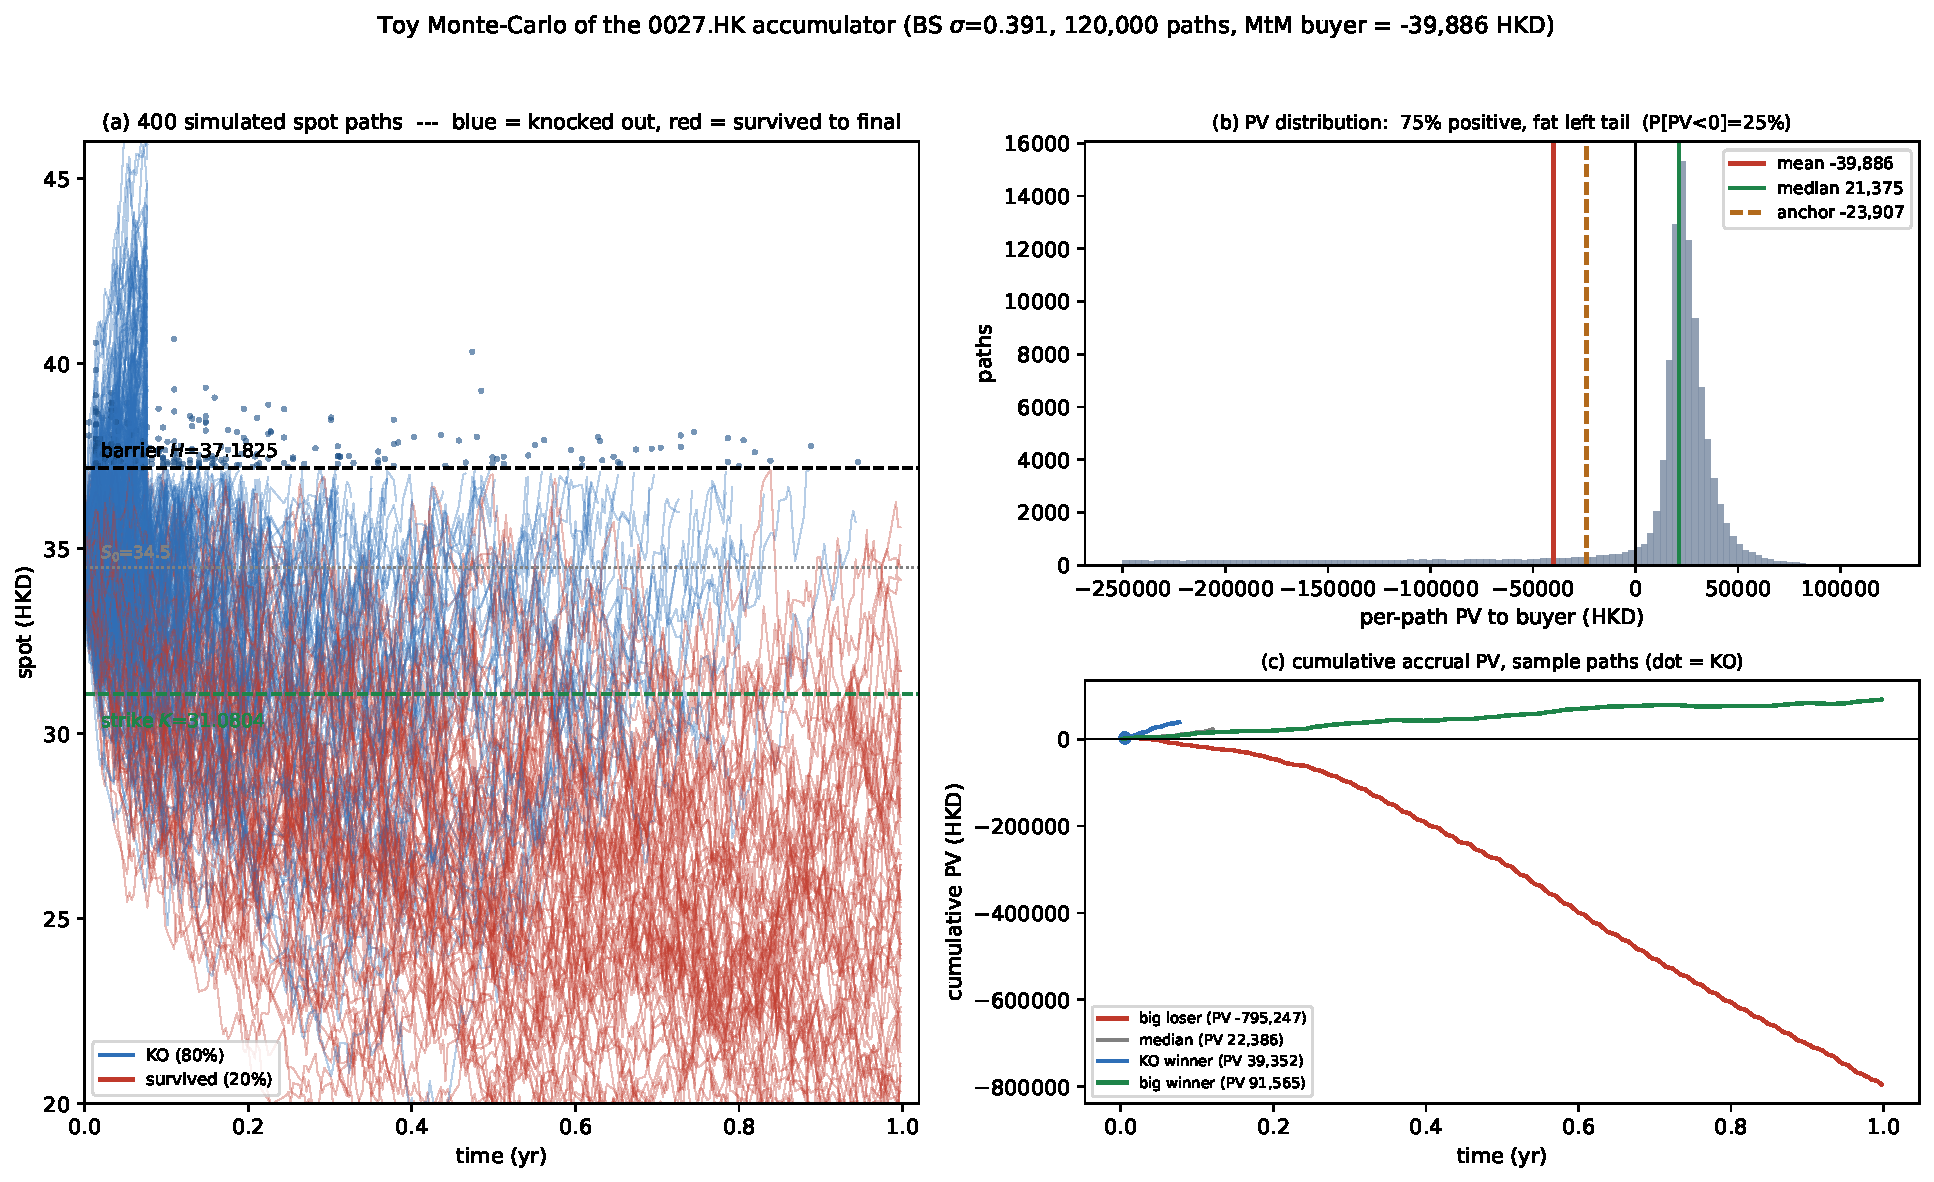
\includegraphics[width=\linewidth]{fig/mc_paths.pdf}
\caption{Toy Monte-Carlo of the accumulator (constant $\sigma=0.391$). \textbf{(a)} spot paths, blue
knocked out and red survived to the final date. \textbf{(b)} the per-path PV, with a positive median
but a negative mean from the fat left tail. \textbf{(c)} cumulative accrual PV for sample paths; a
knocked-out winner stops early, while a downside loser keeps accruing.}
\label{fig:mc}
\end{figure}

% =====================================================================
\section{Volatility Surface and Local Volatility}\label{sec:market}
% =====================================================================
The discount and forward curves are already in place (Section~\ref{sec:data}). This section builds
the two remaining pieces. They are the arbitrage-free volatility surface and the local volatility
fed to the engine.

\subsection{SSVI calibration}
We fit the surface-SVI parametrisation of Gatheral \& Jacquier (2014),
\begin{equation}
  w(k,\theta_T)=\frac{\theta_T}{2}\Bigl\{1+\rho\,\phi\,k+\sqrt{(\phi k+\rho)^2+(1-\rho^2)}\Bigr\},
  \qquad \phi(\theta)=\eta\,\theta^{-\gamma},
\end{equation}
where $w=\sigma_{\mathrm{BS}}^2 T$ is total implied variance and $k=\ln(K/F(T))$ is forward
log-moneyness. Calibration has two steps. First, we read the ATM total-variance term structure
$\theta_T=w(0,T)$. For each expiry $T$ the market gives points $(k_i,w_i)$, with $k_i=\ln(K_i/F(T))$
and $w_i=\sigma_i^2 T$. We interpolate them linearly to $k=0$, then floor the result at the previous
maturity's level:
\begin{equation}
  \theta_T=\max\!\Bigl(\,\underbrace{w_-+\tfrac{-k_-}{\,k_+-k_-\,}\,(w_+-w_-)}_{\text{linear interpolation to }k=0},
  \ \ \theta_{T^-}+\varepsilon\,\Bigr),
  \label{eq:theta}
\end{equation}
where $(k_-,w_-)$ and $(k_+,w_+)$ are the two market points bracketing $k=0$, $T^-$ is the previous
expiry, and $\varepsilon>0$ keeps $\theta_T$ strictly increasing. The floor rules out calendar
arbitrage. Second, we fit the three global smile parameters $(\rho,\eta,\gamma)$ by
Levenberg--Marquardt. We remove the box constraints by reparametrisation. We impose the
Gatheral--Jacquier butterfly conditions $\theta\phi(1+|\rho|)\le4$ and $\theta\phi^2(1+|\rho|)\le4$
as penalty residuals.

\paragraph{Front-window calibration.} The smile $(\rho,\eta,\gamma)$ is a \emph{single global} shape
shared across maturities. Including the long-dated, near-flat slices would flatten it. We therefore
fit only the \textbf{front of the surface}. We use expiries with $T\le1.5\times$ the horizon, about
$1.5$\,yr. These are the eight slices out to about $1.15$\,yr that bracket the one-year contract.
The smile then matches the steep front skew that the barrier actually sees. The fit gives
$\rho\approx+0.15$, a positive (call) skew, with $\eta\approx0.67$ and $\gamma=0.50$. The RMSE is
about $0.0016$ in total variance, or about $0.4$ vol points.

\begin{lstlisting}[language=C++,caption={SSVI calibration (\texttt{ssvi.hpp}).},captionpos=b]
calibrate(surface, market, Tmax):
    theta[0] = 0
    for each expiry T <= Tmax, in increasing order:
        for each market point (moneyness, sigma):
            k = ln(strike / F(T));   w = sigma^2 * T
        theta[T] = max( w(0,T) ,  theta_prev + eps )        // eq. (theta): ATM, non-decreasing

    (rho, eta, gamma) = ( tanh(u0), exp(u1), 0.5/(1+exp(-u2)) )
    minimise over (u0, u1, u2) by Levenberg-Marquardt:
        r  = [ w_SSVI(k, theta(T); rho,eta,gamma) - w   for every quote ]
        r += penalty * max(0, theta*phi   * (1+|rho|) - 4)   at each theta node
        r += penalty * max(0, theta*phi^2 * (1+|rho|) - 4)
    return (rho, eta, gamma, theta)
\end{lstlisting}
\noindent
The reparametrisation keeps $\rho\in(-1,1)$, $\eta>0$ and $\gamma\in(0,\tfrac12)$ without hard
constraints. The butterfly residuals push any no-arbitrage violation back to zero. Figure~\ref{fig:ssvi}
shows the result. The smooth SSVI lines pass through the raw market points, and the smile flattens
with maturity, exactly as $\gamma\to0.5$ predicts.

\begin{figure}[h]\centering
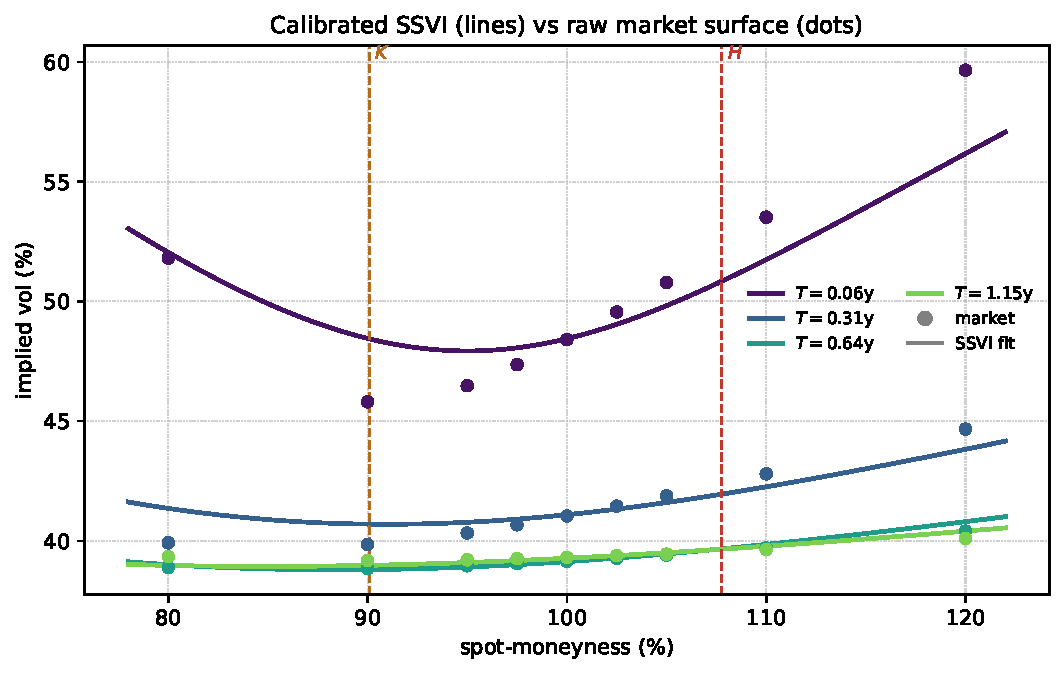
\includegraphics[width=0.82\linewidth]{fig/ssvi_fit.pdf}
\caption{Calibrated SSVI (smooth lines) against the raw \texttt{OVDV} market points (dots), at four
front-window expiries. The arbitrage-free fit smooths the raw grid while preserving the positive
skew. Dashed lines mark the strike $K$ and barrier $H$ in spot-moneyness.}
\label{fig:ssvi}
\end{figure}

\subsection{Dupire local volatility}
Local volatility follows from the calibrated surface by Dupire's formula in Gatheral form,
\begin{equation}
  \sigma_{\mathrm{loc}}^2(S,t)=\frac{\partial_T w}
  {\,1-\dfrac{k}{w}\,\partial_k w+\dfrac14\!\left(-\dfrac14-\dfrac1w+\dfrac{k^2}{w^2}\right)(\partial_k w)^2+\dfrac12\,\partial_{kk}w\,},
  \qquad k=\ln\frac{S}{F(t)},
\end{equation}
We take $\partial_k w$ and $\partial_{kk}w$ analytically from SSVI. We take $\partial_T w$ by a
central difference on the smooth surface. The SSVI no-arbitrage conditions keep the numerator and
denominator positive. So $\sigma_{\mathrm{loc}}$ is well defined over the grid, and we floor it in
the extreme wings for safety. We hand it to the engine as the per-node, per-step $\sigma(S_j,t_k)$.
This is the same Crank--Nicolson code with one vol provider swapped.

\begin{lstlisting}[language=C++,caption={Dupire local volatility from the SSVI fit (\texttt{local\_vol.hpp}).},captionpos=b]
sigma_loc(S, t):
    T = max(t, 1e-4);   k = ln(S / F(T))
    w    = SSVI.w(k, T)
    w_k  = SSVI.dwdk(k, T)                              // analytic
    w_kk = SSVI.d2wdk2(k, T)                            // analytic
    w_T  = ( SSVI.w(k, T+h) - SSVI.w(k, T-h) ) / (2h)   // central difference
    denom = 1 - (k/w)*w_k + (1/4)*(-1/4 - 1/w + k*k/(w*w))*w_k*w_k + (1/2)*w_kk
    return sqrt( max( w_T / denom , vol_floor^2 ) )
\end{lstlisting}

% =====================================================================
\section{Results}\label{sec:results}
% =====================================================================
We now run the engine on the trade-date market of Section~\ref{sec:data}. It returns the buyer PV
under both models (Table~\ref{tab:results}).

\begin{table}[h]\centering\small
\begin{tabular}{@{}lr@{}}
\toprule
Model & Buyer PV (HKD) \\
\midrule
Black--Scholes (vol at strike) & $-39{,}879$ \\
Local volatility (SSVI / Dupire) & $-45{,}956$ \\
\midrule
Trade-date anchor (initial exchange) & $-23{,}906$ \\
\bottomrule
\end{tabular}
\caption{Buyer PV under Black--Scholes and local volatility, versus the trade-date anchor.}
\label{tab:results}
\end{table}

\paragraph{Local vs Black--Scholes.} Local volatility is \emph{more} negative than flat
Black--Scholes here. The calibrated surface has a \emph{positive} (call) skew, $\rho\approx+0.15$. The barrier sits at about $108\%$ of spot. It
therefore carries implied volatility above the at-the-money level, and hence higher local
volatility. Higher volatility at the barrier raises the knock-out probability. This removes more of
the buyer's positive accrual and pushes the PV down.

\paragraph{Validation against the anchor.} The term sheet's \emph{Initial Exchange Amount} is HKD
$23{,}906.61$, payable by Citigroup to the buyer, but our PDE engine returns a much more negative PV. We verified our engine against the closed form in Section~\ref{sec:analytic}. The engine is therefore correct. We also use a toy Monte-Carlo pricer to cross-check the results. It demonstrates the same pattern.The gap probably reflects bid-ask spreads on this structure.

% =====================================================================
\section{Greeks and Risk}\label{sec:greeks}
% =====================================================================
The engine gives the first-order Greeks almost for free. We read Delta and Gamma straight off the
as-of value surface. In log-spot, $\Delta=\partial_x W/S$ and $\Gamma=(\partial_{xx}W-\partial_x W)/S^2$
at the spot node, from adjacent grid values. This is one solve and no re-pricing. Vega is different.
Volatility is a model parameter, not a grid axis, so we cannot read it off the surface. We instead
bump the vol by one point and re-solve. Table~\ref{tab:greeks} collects the results.

\begin{table}[h]\centering\small
\begin{tabular}{@{}lrrl@{}}
\toprule
Greek & Black--Scholes & Local vol & source \\
\midrule
Delta $\partial V/\partial S$      & $24{,}179$ & $22{,}964$ & grid \\
Gamma $\partial^2 V/\partial S^2$  & $-1{,}732$ & $-13{,}893$ & grid \\
Vega (per vol point)               & $-2{,}220$ & $-2{,}525$ & bump $\pm1$\,vp \\
\bottomrule
\end{tabular}
\caption{As-of Greeks to the buyer. Delta and Gamma are read off the PDE grid; Vega is a
$\pm1$-vol-point bump-and-revalue.}
\label{tab:greeks}
\end{table}

We validate the grid read by bump-and-revalue. We bump the spot by $\pm0.25\%$, re-solve with the
local-vol field held fixed, and difference the prices. The grid and bumped Delta agree to $0.3\%$
($22{,}964$ vs $22{,}891$). The grid and bumped Gamma agree to $0.4\%$ ($-13{,}893$ vs $-13{,}837$).
The small bump matters for Gamma. Gamma is sharp near the barrier, so a coarser bump smooths it away;
the grid read resolves it at the finest step.

The signs tell the risk story. Delta is large and positive, about $+23{,}000$. The buyer is long the
underlying, because it accrues shares. Gamma is negative, about $-13{,}900$ under local vol. The
buyer is short Gamma, because the knock-out caps the upside and makes the value concave. Vega is
negative, about $-2{,}500$ per vol point. The buyer is short volatility. This matches the
short-volatility, fat-tail picture of Section~\ref{sec:analytic}.

Figure~\ref{fig:greeks} shows where the risk lives. Delta declines smoothly, then drops sharply at
the barrier. Gamma is small away from the barrier but explodes at $H$. The local-vol Gamma is far
larger in magnitude than the Black--Scholes Gamma, because the surface carries high volatility at the
barrier. The risk is concentrated at the knock-out. That is exactly where a finite-difference grid
resolves it best, and it is the main reason we chose a PDE.

\begin{figure}[h]\centering
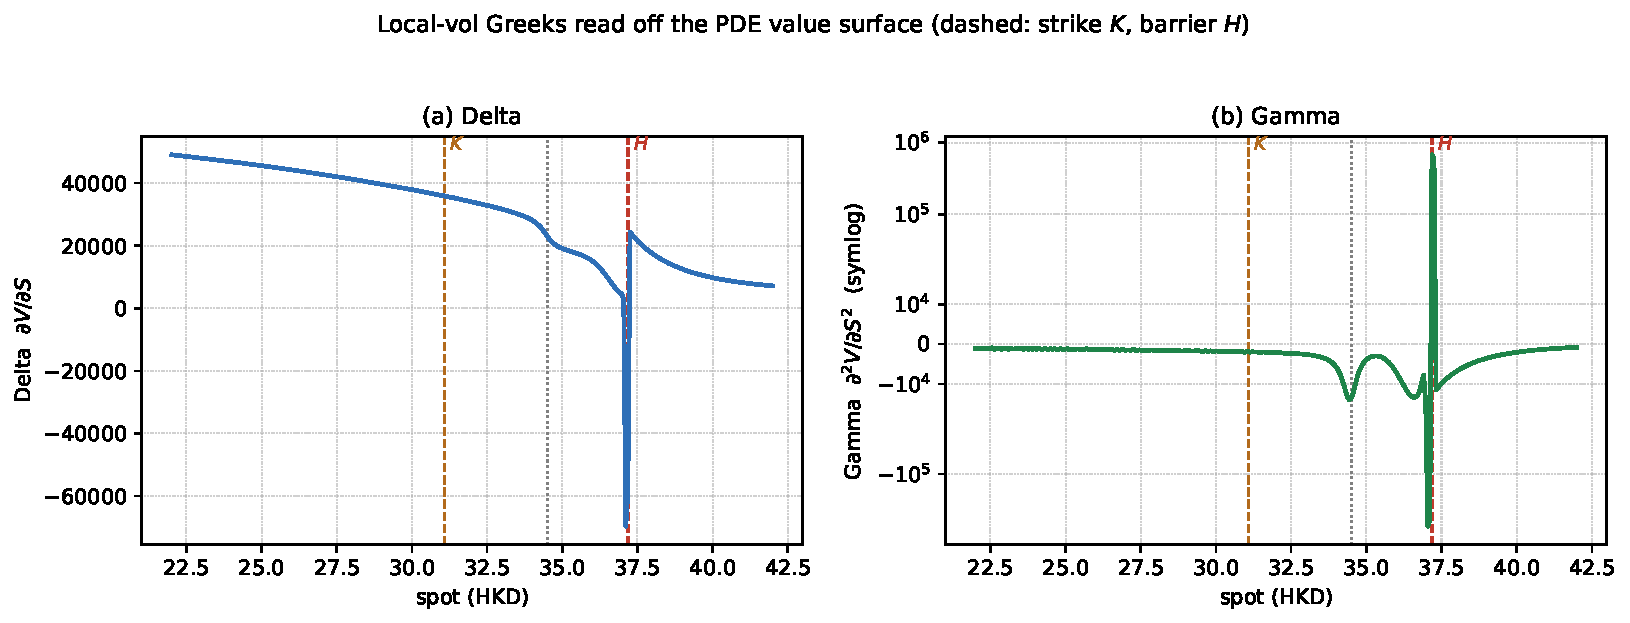
\includegraphics[width=\linewidth]{fig/greeks.pdf}
\caption{Local-vol Delta and Gamma across spot, read off the as-of PDE value surface. Delta has a
cliff at the barrier $H$; Gamma (symlog scale) is small away from $H$ and singular at $H$. Dashed
lines mark the strike $K$ and barrier $H$.}
\label{fig:greeks}
\end{figure}

% =====================================================================
\section{Conclusion}
% =====================================================================
The accumulator is Markovian in the single underlying. A one-dimensional Crank--Nicolson PDE is
therefore the natural pricer. It treats the daily discrete barrier exactly. It absorbs the
guaranteed period and the accrual cap. It also delivers clean Greeks where the risk concentrates.
We validated the engine against an independent closed-form benchmark. Under a matched constant
volatility, the PDE converges to the exact Reiner--Rubinstein price in the continuous-monitoring
limit. We then built the market-data and local-volatility layer (Section~\ref{sec:market}) and
priced the real trade (Section~\ref{sec:results}). Finally, we read the Greeks off the same value
surface and validated them by bump-and-revalue (Section~\ref{sec:greeks}). The buyer holds a long
Delta, short Gamma, and short Vega position, with the risk concentrated at the barrier.

\appendix
% =====================================================================
\section{Row-wise expansion of the Crank--Nicolson system}\label{app:cn}
% =====================================================================
Consider the matrix form \eqref{eq:cn-matrix}. Here $W^{k}$ and $W^{k+1}$ are \emph{vectors} over
the $N_x{+}1$ grid nodes. The operator $\Lh$ is the tridiagonal \emph{matrix} with rows
$(\ell_j,d_j,u_j)$ from \eqref{eq:Lcoeffs}. The symbol $I$ is the identity, and $A=\tfrac12\Delta t$
is a scalar. The equation is thus ``matrix $\times$ vector $=$ vector'', one scalar equation per
node $j$. Acting on a vector, row $j$ of the operator is
\begin{equation}
  (\Lh W)_j \;=\; \ell_j W_{j-1} + d_j W_j + u_j W_{j+1}.
\end{equation}

\paragraph{Left-hand side.} Row $j$ of $(I-A\Lh)W^{k}$ (the unknowns) is
\begin{align}
  \bigl[(I-A\Lh)W^{k}\bigr]_j
   &= W_j^{k} - A\bigl(\ell_j W_{j-1}^{k}+d_j W_j^{k}+u_j W_{j+1}^{k}\bigr)\nonumber\\
   &= \underbrace{(-A\ell_j)}_{\texttt{a[j]}}\,W_{j-1}^{k}
    + \underbrace{(1-Ad_j)}_{\texttt{b[j]}}\,W_{j}^{k}
    + \underbrace{(-Au_j)}_{\texttt{c[j]}}\,W_{j+1}^{k}.
\end{align}
The $1$ in the diagonal entry $1-Ad_j$ is the contribution of the identity $I$.

\paragraph{Right-hand side.} Row $j$ of $(I+A\Lh)W^{k+1}$ uses only the known level $W^{k+1}$. It
therefore evaluates to a number:
\begin{equation}
  \texttt{rhs[j]} \;=\; W_j^{k+1} + A\bigl(\ell_j W_{j-1}^{k+1}+d_j W_j^{k+1}+u_j W_{j+1}^{k+1}\bigr).
\end{equation}

\paragraph{The system.} Collecting rows gives one tridiagonal equation per node,
\begin{equation}
  -A\ell_j\,W_{j-1}^{k} + (1-Ad_j)\,W_j^{k} - Au_j\,W_{j+1}^{k} \;=\; \texttt{rhs[j]},
\end{equation}
i.e.\ the banded system (interior rows shown)
\begin{equation}
\footnotesize
\begin{pmatrix}
1{-}Ad_0 & -Au_0 & & & \\
-A\ell_1 & 1{-}Ad_1 & -Au_1 & & \\
 & \ddots & \ddots & \ddots & \\
 & & -A\ell_{N_x-1} & 1{-}Ad_{N_x-1} & -Au_{N_x-1}\\
 & & & -A\ell_{N_x} & 1{-}Ad_{N_x}
\end{pmatrix}
\!\!
\begin{pmatrix} W_0^{k}\\[1pt] W_1^{k}\\[1pt] \vdots\\[1pt] W_{N_x-1}^{k}\\[1pt] W_{N_x}^{k}\end{pmatrix}
\!=\!
\begin{pmatrix} \texttt{rhs[0]}\\[1pt] \texttt{rhs[1]}\\[1pt] \vdots\\[1pt] \texttt{rhs[$N_x{-}1$]}\\[1pt] \texttt{rhs[$N_x$]}\end{pmatrix},
\end{equation}
We solve it for $W^{k}$ in $O(N_x)$ by the Thomas algorithm. The boundary rows $j=0,N_x$ use the
linear far-field ($W_{xx}=0$) stencil of Section~\ref{sec:framework} in place of the interior
$(\ell,d,u)$. The arrays \texttt{a}, \texttt{b}, \texttt{c}, \texttt{rhs} are exactly those in
\texttt{pde\_engine.hpp}.

% =====================================================================
\section{Reiner--Rubinstein building blocks}\label{app:rr}
% =====================================================================
With $\phi=\pm1$ (call/put), $\eta=\pm1$ (down/up), carry $b=r-q$, $\mu_H=(b-\tfrac12\sigma^2)/\sigma^2$,
$x_1=\tfrac{\ln(S/X)}{\sigma\sqrt t}+(1+\mu_H)\sigma\sqrt t$,
$x_2=\tfrac{\ln(S/H)}{\sigma\sqrt t}+(1+\mu_H)\sigma\sqrt t$,
$y_1=\tfrac{\ln(H^2/SX)}{\sigma\sqrt t}+(1+\mu_H)\sigma\sqrt t$,
$y_2=\tfrac{\ln(H/S)}{\sigma\sqrt t}+(1+\mu_H)\sigma\sqrt t$:
\begin{align}
A &= \phi S e^{(b-r)t}\Phi(\phi x_1) - \phi X e^{-rt}\Phi(\phi x_1-\phi\sigma\sqrt t),\\
B &= \phi S e^{(b-r)t}\Phi(\phi x_2) - \phi X e^{-rt}\Phi(\phi x_2-\phi\sigma\sqrt t),\\
C &= \phi S e^{(b-r)t}(H/S)^{2(\mu_H+1)}\Phi(\eta y_1) - \phi X e^{-rt}(H/S)^{2\mu_H}\Phi(\eta y_1-\eta\sigma\sqrt t),\\
D &= \phi S e^{(b-r)t}(H/S)^{2(\mu_H+1)}\Phi(\eta y_2) - \phi X e^{-rt}(H/S)^{2\mu_H}\Phi(\eta y_2-\eta\sigma\sqrt t).
\end{align}
For $X<H$: up-and-out call $=A-B+C-D$ ($\phi{=}1,\eta{=}{-}1$); up-and-out put $=A-C$
($\phi{=}{-}1,\eta{=}{-}1$). Here $\Phi$ is the standard normal CDF.

% =====================================================================
\section{Implementation}\label{app:impl}
% =====================================================================
The engine is a header-only C++20 library (\texttt{github.com/Zale1516/equity\_pricer}). Python
tools build the JSON inputs from Bloomberg exports. They write \texttt{market\_data.json}, which
holds the discount and forward curves and the vol surface, and \texttt{trade.json}. The C++ engine
ingests both. The key files are \texttt{pde\_engine.hpp} (Crank--Nicolson),
\texttt{analytic\_engine.hpp} (Reiner--Rubinstein and BGK), \texttt{market.hpp},
\texttt{vol\_surface.hpp}, and \texttt{accumulator.hpp}.

% =====================================================================
\section*{References}
\addcontentsline{toc}{section}{References}
% =====================================================================
\begin{list}{}{\setlength{\leftmargin}{1.6em}\setlength{\itemindent}{-1.6em}\setlength{\itemsep}{3pt}}
\item Broadie, M., Glasserman, P., \& Kou, S. (1997). A continuity correction for discrete barrier
      options. \emph{Mathematical Finance}, 7(4), 325--349.
\item Gatheral, J., \& Jacquier, A. (2014). Arbitrage-free SVI volatility surfaces.
      \emph{Quantitative Finance}, 14(1), 59--71.
\item Lam, K., Yu, P., \& Xin, L. (2009). Accumulator pricing. \emph{IEEE Symposium on
      Computational Intelligence for Financial Engineering (CIFEr)}.
\item Reiner, E., \& Rubinstein, M. (1991). Breaking down the barriers. \emph{Risk}, 4(8), 28--35.
\end{list}

\end{document}
